
Voici la courbe de poids du petit Paul de sa naissance jusqu'à l'âge de 9 semaines.

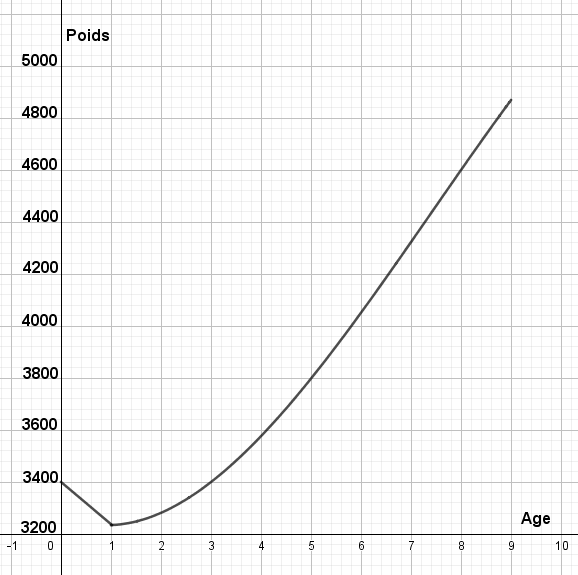
\includegraphics[scale=1]{VF-26.png} 


\begin{enumerate}
\item Déterminer les unités de chacun des axes.
\item Le pédiatre commente la courbe aux parents légèrement inquiets. Compléter ses propos.

"Il est normal qu'après la naissance le poids diminue pendant .............\\

Votre bébé a retrouvé son poids\footnote{Dans le langage courant, on assimile le poids à la masse, ce qui est une erreur en Sciences Physiques.} de naissance au bout de ........................... ce qui est tout a fait habituel.\\

Sa croissance est même désormais de plus en plus rapide, il suffit de regarder de la 4è à la 5è semaine il n'a pris que

 ................... environ alors que de la 7è à la 8è semaine il a pris environ ...............\\

A partir de la ......................., son poids a dépassé 4600 .............."
\item Justifier que son poids à 5 semaines est supérieur à son poids à 4 semaines.
\item Dresser le tableau de variations de cette fonction sur l'intervalle $[0;8]$. Quel a été le poids minimal de Sacha ?
\item Un bébé peut perdre jusqu'à 10\% de son poids après la naissance. Y a-t-il lieu de s'inquiéter pour Sacha ?



\end{enumerate}
